\documentclass[a4paper,10pt]{article}
\usepackage[margin=15mm]{geometry}
\usepackage{pgf,tikz}
\usepackage{algorithm2e}
\usepackage{subfig}
\usepackage{amsmath}
\usepackage{color}
\usepackage{amssymb}
\usepackage{noweb}
\usepackage{listings}
\usetikzlibrary{circuits.logic.US}
\usetikzlibrary{positioning}
\usetikzlibrary{matrix}
 
\definecolor{dkgreen}{rgb}{0,0.6,0}
\definecolor{gray}{rgb}{0.5,0.5,0.5}
\definecolor{mauve}{rgb}{0.58,0,0.82}

\lstset{ %
  language=Verilog,                % the language of the code
  basicstyle=\footnotesize,           % the size of the fonts that are used for the code
  numbers=left,                   % where to put the line-numbers
  numberstyle=\tiny\color{gray},  % the style that is used for the line-numbers
  stepnumber=2,                   % the step between two line-numbers. If it's 1, each line 
                                  % will be numbered
  numbersep=5pt,                  % how far the line-numbers are from the code
  backgroundcolor=\color{white},      % choose the background color. You must add \usepackage{color}
  showspaces=false,               % show spaces adding particular underscores
  showstringspaces=false,         % underline spaces within strings
  showtabs=false,                 % show tabs within strings adding particular underscores
%  frame=single,                   % adds a frame around the code
  rulecolor=\color{black},        % if not set, the frame-color may be changed on line-breaks within not-black text (e.g. commens (green here))
  tabsize=2,                      % sets default tabsize to 2 spaces
  captionpos=b,                   % sets the caption-position to bottom
  breaklines=true,                % sets automatic line breaking
  breakatwhitespace=false,        % sets if automatic breaks should only happen at whitespace
  title=\lstname,                   % show the filename of files included with \lstinputlisting;
                                  % also try caption instead of title
  keywordstyle=\color{blue},          % keyword style
  commentstyle=\color{dkgreen},       % comment style
  stringstyle=\color{mauve},         % string literal style
  escapeinside={\%*}{*)},            % if you want to add LaTeX within your code
  morekeywords={*,...}               % if you want to add more keywords to the set
}
\usepackage{amsthm}
\usepackage{hyperref}
\setlength{\parskip}{3mm}
\newtheorem{axiom}{Axiom}
\newtheorem{definition}{Definition}
\newtheorem{comment}{Comment}
\newtheorem{example}{Example}
\newtheorem{lemma}{Lemma}
\newtheorem{prop}{Property}
\newtheorem{problem}{Problem}
\newtheorem{remark}{Remark}
\newtheorem{theorem}{Theorem}

% Title Page
\title{EE677 : \textbf{Foundation of VLSI CAD} \\
Comments on project problems}
\author{Dilawar Singh}
\date{Sep 22, 2012}

\begin{document}
\maketitle

\begin{abstract}

  This document partly describes many of the problems listed on course wiki.
  This is not a technical document which explains problems in details.
  Algorithms used to tackle these problems can be found in two books :
  \textbf{Introduction to algorithms}, Cormen, Leiserson et. al.  which deals
  with algorithms in general; and \textbf{Graph Theory} with application to
  Engineering and Computer Science by Narsing Deo, which explains graph
  algorithms lucidly.

  Algorithms related with placement and routing, circuit partitioning, layout
  generation in the area of VLSI CAD can be found in \textbf{VLSI Physical
  Automation} by Sadiq M Sait et. al.. 

  It is hard to say how much effort is precisely needed to solve problems listed
  in this document. It depends as much on your fluency with programming language
  as it depends on theoretical understanding. However, I have mentioned an
  integer in front of some problems which roughly indicates the effort needed to
  solve them. Needless to say, this number can be well wide off the mark.

\end{abstract}

\section{Graphs in Boolean world}
\label{sec:data_structure}

\begin{flushright}
  As an old Chinese philosopher never said, "Words about graphs are \\ worth a
  thousand pictures." \\ 
  -- \textbf{William Saffire}, \emph{The English Language} \\
  The New York Times, Sep 11, 2009
\end{flushright}

\paragraph{Lobbying for graphs}

  Data-structures such as array, list, vector, map, dictionary etc. are very
  useful. However, graphs has its own place among the titans.  Many
  algorithms become easier to visualize when we make use of graphs on paper;
  proofs are easy to state and understand. 

  Moreover, from the point of view of a programmer, coding with graph is
  convenient since sophisticated graph libraries are available in almost all
  self-respecting languages. Of course, there is a price to pay for this
  convenience : graphs consume relatively more memory to construct. Where
  available memory size is limited, such as on embedded systems, one may not be
  able to use graphs. One has to rewrite his algorithm which works on less costly
  data-structures.

  In 1975, there was only one book available on graph theory. It was written by
  Koing in German (\texttt{Theorie der Endlichen und Unendlichen Graphen}).
  (Later, William Tutte translated this book into English.) In
  its early years, graph theory was often looked upon with condescend by some
  mathematician. "The slum of topology" was the derisive remark they used to pass. 

  Since then graphs has emerged out of "the slum of topology" to become one of
  the most extensively studied mathematical structure.

  Narsingh Deo book "\textbf{Graph theory} with applications to engineering and
  computer science" is a very good introductory book on graph-theory for
  engineers. H. Narayan's "Submodular function and Electrical Network",
  especially chapter 3, gives an excellent overview of graphs in networks.
  
\paragraph{Libraries}

  There are many graph libraries available. No language which claims to be a
  contender for algorithmic design can exists without a graph library. We
  recommend using \textbf{Boost libraries} or \textbf{LEDA graph libraries} for
  C++. Boost graph libraries bindings are available for python, package
  \textbf{graph-tool}.  Python's native graph library \textbf{networkx} can also
  be used for small graph applications. Networkx has great many routines but it
  is not recommended for very large graphs for speed of networkx is not very
  good compared to graph-tool.

\paragraph{String graph to files}

   Format \textbf{dot} and \textbf{graphml} are two modern graph-formats. We'll
   use graphml to encode/decode our graph to a file. Both boost and LEDA
   libraries can read and write graphs to graphml format. This is a text-based
   format and can be read by humans.

\subsection{Graph as Boolean expression trees}

    In many of these project problems, we'll be working with Boolean expressions
    as input to the program or as intermediate data.  There are many ways to
    feed a Boolean expressions to a computer program. We need to fix a standard
    such that data can be transferred from one program to another without any
    hassle. 

    Boolean expressions can be encoded as expression-trees. What are expression
    trees? Mimicking Dodo the bird of 'Alice in Wonderland', one is temped to
    conclude that the best way to explain it is to show it. 

    On paper, Boolean expressions are written using standard symbols.  Table
    \ref{table:symbols} summarises them.

    \begin{figure}[h]
      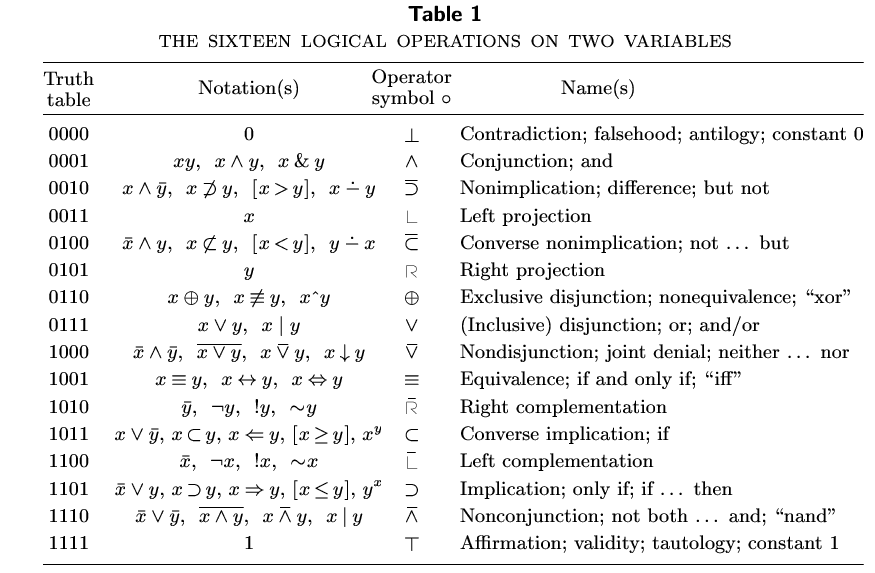
\includegraphics[width=\textwidth]{./figs/symbols.png}
      \caption{\small From Knuth, TAOP, 4A}
      \label{table:symbols}
    \end{figure}
    
    Consider the following expression. We are using standard Boolean symbols in these
    expressions.

    \begin{equation}
    \label{eq:expr1}
    y = (x_1 \vee x'_2) \wedge (x_2 \vee x_3) \wedge (x'_1 \vee x'_3)
    \end{equation}

    \begin{figure}[h]
    \centering
    \subfloat[]{
    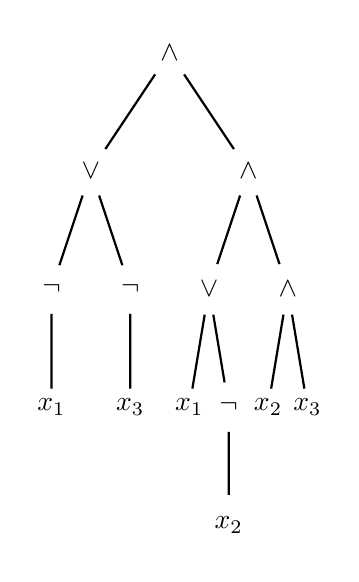
\begin{tikzpicture}
    [level distance = 15mm, thick,
      every node/.style={circle},
      level 1/.style={sibling distance=20mm,}, %
      level 2/.style={sibling distance=10mm,}, % nodes={fill=red!20}},
      level 3/.style={sibling distance=5mm,}, % nodes={fill=red!10}}
     ]
    \node {$\wedge$}
    child {node {$\vee$}
      child {node {$\neg$}
        child {node[rectangle] {$x_1$}}
       }
      child {node {$\neg$}
        child {node[rectangle] {$x_3$}}
       }
    }     
    child {node {$\wedge$}
      child {node {$\vee$}
        child {node[rectangle] {$x_1$}}
        child {node {$\neg$}
          child {node {$x_2$}}
         }
      }
      child {node {$\wedge$}
        child {node [rectangle] {$x_2$}}
        child {node [rectangle] {$x_3$}}
       }
     }
      ;
    \end{tikzpicture}
    }
    \subfloat[]{
    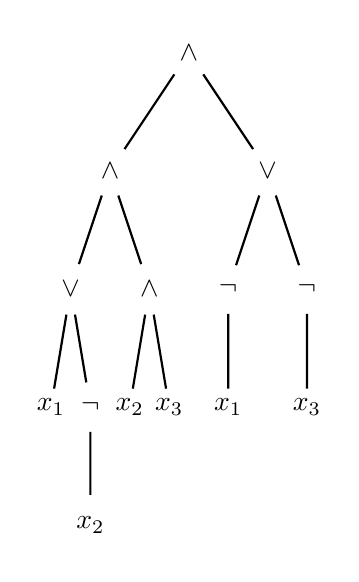
\begin{tikzpicture}
    [level distance = 15mm, thick,
      every node/.style={circle},
      level 1/.style={sibling distance=20mm,}, %
      level 2/.style={sibling distance=10mm,}, % nodes={fill=red!20}},
      level 3/.style={sibling distance=5mm,}, % nodes={fill=red!10}}
     ]
    \node {$\wedge$}
     child {node {$\wedge$}
      child {node {$\vee$}
        child {node[rectangle] {$x_1$}}
        child {node {$\neg$}
          child {node {$x_2$}}
         }
      }
      child {node {$\wedge$}
        child {node [rectangle] {$x_2$}}
        child {node [rectangle] {$x_3$}}
       }
     }
    child {node {$\vee$}
      child {node {$\neg$}
        child {node[rectangle] {$x_1$}}
       }
      child {node {$\neg$}
        child {node[rectangle] {$x_3$}}
       }
    }     
    ;
    \end{tikzpicture}
   }

   \caption{Two possible expression-trees of Boolean expression described in
     equation \ref{eq:expr1}. Some other representations are also possible.
     Since we have proved associativity in Boolean algebra, both of these trees
     are functionally equivalent. Although it is not at all easy to show that
     two given  expression trees are functionally equivalent or not.}
   \label{fig:expr_tree} 
 
 \end{figure}

    We'll use \texttt{not}, \texttt{and}, \texttt{or} to describe gates while
    writing these expressions. In special cases, such as technology mapping, one
    can also use additional \texttt{xor}, \texttt{nor}, and \texttt{nand} in
    output graph \footnote{A detailed standard should be made available on
      wiki}.  Figure \ref{fig:expr_tree} encodes these expression into an
    expression tree.
  

Three problems are immediate.
  
  \begin{problem}[15]
  \label{prob:expr_tree_to_minterms}
  Given a Boolean expression tree, construct another graph where each node
  represents a minterm of function. And an edge is drawn between two nodes whenever
  their Hamming distance is 1.
\end{problem}

  Such a graph could be an input to Quine McClusky algorithm which works over
  graphs (as we have discussed during project-session).

  \begin{problem}[25]
  \label{prob:minimize_expression_tree}
  Given a Boolean expression tree, minimize the Boolean function represented.
  \ref{prob:expr_tree_to_minterms}.   
  
  \end{problem}

  \begin{problem}[45]
  \label{prob:equivalence_checking}
  Given two Boolean expression trees, check if both expressions trees represents
  same Boolean function or not.
  \end{problem}


  \begin{remark}[HDL to Boolean expression-trees]

    Is there any way to construct Boolean expression tree out of a verilog
    design? Well, there seems to be one and TA of this course should give you a
    program to do this.

    Computer program \textbf{vis} can convert a verilog design to a
    \textbf{bliff} file. All we have to do is to convert this bliff file into
    boolean expression tree. 
  
  \end{remark}


\newpage
\subsection{Graphs as Binary Decision Diagrams}

\begin{flushright}

In popular usage, the term BDD almost always refers to Reduced Ordered Binary
Decision Diagram (ROBDD in the literature, used when the ordering and reduction
aspects need to be emphasized). The advantage of an ROBDD is that it is
canonical (unique) for a particular function and variable order. This
property makes it useful in functional equivalence checking and other operations
like functional technology mapping. \\
-- \textbf{Wikipedia}, The free encyclopedia (Accessed Sep 22, 2012) 

\end{flushright}

  One more way to encode a Boolean expression is BDD (Binary Decision
  Diagrams) which can been seen as recursive composition of
\textbf{If-then-else} logic.

  \paragraph{If-Then-Else}
  A Boolean function $f(x_1,\ldots,x_n)$ can be decomposed as following :
  \begin{equation}
    \begin{gathered}
      \begin{aligned}
        f(x_1,\ldots,x_n) &= {x'_1} \vee g(x_2,\ldots,x_n) \wedge {x_1} \vee
        h(x_2,\ldots,x_n), \text{where} \\
        g(x_2,\ldots,x_n) &= f(0,x_2,\ldots,x_n) \\
        h(x_2,\ldots,x_n) &= f(1,x_2, \ldots, x_n) \\
      \end{aligned}
    \end{gathered}
  \end{equation}

  This can be read as (ignoring function argument) : \textbf{if} $x_1=0$
  \textbf{then} $f = g$ \textbf{else} $f=h$. For electrical engineer, it is well
  known multiplexer. 


  \begin{figure}[h]
    \centering
    \subfloat[Mux]{
    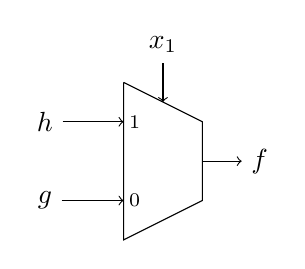
\begin{tikzpicture}[circuit logic US]
      %% Dilawar Singh (c) 2012 
%% Circuit macros to produce amazing quality macros. More amazing and powerpuff
%% girls.
\def\mux { -- ++(0,-1) node [above right] {$1$} -- ++(0.6,0.2) -- 
++(0,0.6) -- ++(-0.6,0.2) -- cycle};
\def\muxr { -- node [below left] {$1$} ++(1,0) -- ++(-0.2,-0.6) -- 
++(-0.6,0) -- ++(-0.2,0.6)  -- cycle};

%% Multiplexor 
%% 3 params : location, size, name.
%% Note : To connect wires to north, east, south and west one should 
%% also use .center with name.
\newcommand{\multiplexer}[3]{
\draw #1 -- ++(0,-#2/4)  node (#3_input1) at ++(0,0) {\scriptsize{\hspace{8pt}1}}
-- ++(0,-#2/2) node (#3_input2) at ++(0,0){\scriptsize{\hspace{8pt}0}} 
-- ++(0,-#2/4) -- ++(#2/2,#2/4)
-- ++(0,#2/4) node(#3_output) [] {}  -- ++(0,#2/4) 
-- ++(-#2/4,#2/8) node(#3_select) {} -- ++(-#2/4,#2/8)
};

%% Register 
%% 4 parama : location, width, height, name 
%% Note : To connect wires to north, east, south and west one should 
%% also use .center with name.
\newcommand{\register}[4]{
\draw #1 -- ++(#2/2,0) node(#4_north){} --++(#2/2,0) 
% eastern side
-- ++(0,-#3/2) node(#4_east){} -- ++(0,-#3/2) 
% southern side 
-- ++(-#2/2,0) node(#4_south){} --++(-#2/2,0) 
% label 
-- ++(0,#3) node at ($#1+(#2/2+0.1,-#3/2)$) {#4} 
% the western triangle
-- ++(0.6*#3, -0.5*#3) -- ++(-0.6*#3, -0.5*#3)
% the western anchor
-- ++(0,#3/2) node (#4_west) {} 
};

%% Bus
%% 3 params : from, to, size 
\newcommand*{\bus}[4] {
\draw[->] #1 -- #2 node[midway]{\tiny{/}} 
    node [#3] {\scriptsize{#4}}
}

      \multiplexer{(2,0)}{2}{a};
      \node (h) at (1,-0.5) {$h$};
      \node (g) at (1,-1.5) {$g$};
      \draw[->] (h) -- (a_input1.center);
      \draw[->] (g) -- (a_input2.center);
      \draw[<-] (a_select.center) -- ++(0,0.5) node[above] {$x_1$};
      \draw[->] (a_output.center) -- ++(0.5,0) node[right] {$f$};
    \end{tikzpicture}
  }
  \subfloat[Graph of $f$]{
    \begin{tikzpicture}
      \node {$x_1$} 
        child[dotted] {node {$g$}}
        child {node {$h$}}
        ;
    \end{tikzpicture}
  }
  \caption{\textbf{If-Then-Else} operator. In (a) we have corrosponding
  circuit, which is a mux. In (b), we have graphical representation of
  $f$. Dotted line indicates that on this branch $x_1=0$.}
  \end{figure}

  Variable $x_1$ does not appear in $g$ and $h$. One application of
\textbf{if-then-else} breaks a function on $n$ variables into two functions of
$n-1$ variables. We can apply \textbf{if-then-else} operator recursively till
we are left with constant function $0$ and $1$. Lets consider the following
expression.

    \begin{equation}
    \label{eq:expr2}
    y = (x_1 \vee x'_2) \wedge (x_2 \vee x_3) 
    \end{equation}

   Now, we can construct a diagram which shows the process of recursively
   applying the \textbf{if-then-else}. This process is illustrated below.

   \begin{figure}[h]
     \centering
     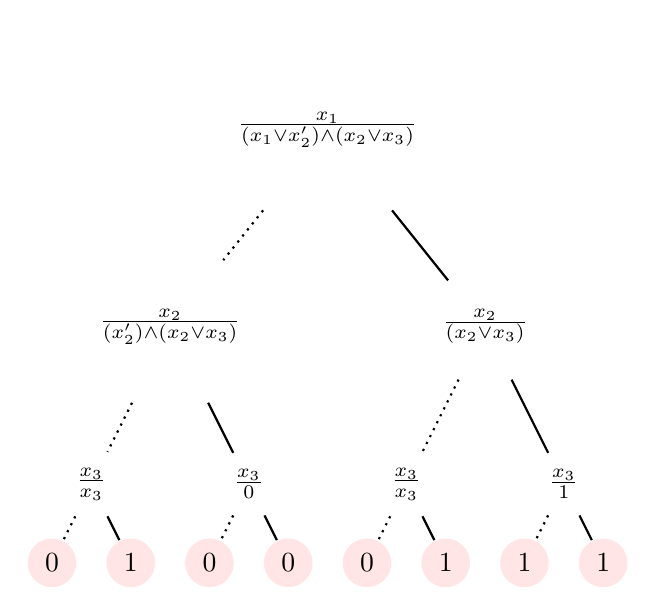
\begin{tikzpicture}
      [ 
        every node/.style={circle}, thick,
        level 1/.style={sibling distance=40mm, level distance=25mm,}, %
        level 2/.style={sibling distance=20mm, level distance=20mm,}, % nodes={fill=red!20}},
        level 3/.style={sibling distance=10mm, level distance=10mm
        ,nodes={fill=red!10}}
      ]
      \node {$\frac{x_1}{(x_1 \vee x'_2) \wedge (x_2 \vee x_3)}$}
        child[dotted] {node {$\frac{x_2}{(x'_2) \wedge (x_2 \vee x_3)}$}
          child[dotted] {node {$\frac{x_3}{ x_3}$}
            child[dotted] {node {$0$}}
            child[solid] {node {$1$}}
          }
          child[solid] {node {$\frac{x_3}{0}$}
            child[dotted] {node {$0$}}
            child[solid] {node {$0$}}
          }
        }
        child[] {node {$\frac{x_2}{(x_2 \vee x_3)}$}
          child[dotted] {node {$\frac{x_3}{x_3}$}
            child[dotted] {node {$0$}}
            child[solid] {node {$1$}}
          }
          child[] {node {$\frac{x_3}{1}$}
            child[dotted] {node {$1$}}
            child[solid] {node {$1$}}
          }
        }
       ;
     \end{tikzpicture}

     \caption{\small A graph diagram represents function described in equation
     \ref{eq:expr2}. A network of mux can be built form this graph. This kind of
   graph are called Binary Decision Diagrams. Usually reduced expression is not
   written below the variable name as we have written in this diagram.}
   
   \end{figure}

   A cursory look will reveal that this is very inefficient. We don't need so
   many nodes for $0$ and $1$. One node for each of them will suffice which can
   be shared by multiple edges by other nodes. Other simplifications are also
   possible which are discussed at length in your textbook.  Verify that
   following diagram also encode the same function but with fewer nodes. 

   \begin{figure}[h]
    \centering
    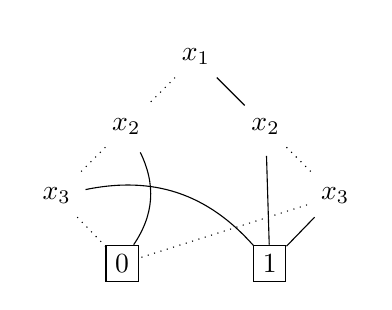
\begin{tikzpicture}
      [ node distance=5mm
        , every node/.style={}
      ]
      \node (x1) [, circle] {$x_1$};
      \node (x21) [circle, , below right=of x1] {$x_2$};
      \node (x20) [circle, , below left=of x1] {$x_2$};
      \draw[dotted] (x1) -- (x20);
      \draw[] (x1) -- (x21);
      \node (x30) [circle, , below left=of x20] {$x_3$};
      \node (x31) [circle, , below right=of x21] {$x_3$};
      \node (b0) [rectangle, draw , below right=of x30] {$0$};
      \node (b1) [rectangle, draw , below left=of x31] {$1$};

      \draw[dotted] (x20) -- (x30); 
      \draw (x20) to [bend left] (b0);
      \draw[] (x21) to [] (b1);
      \draw[dotted] (x21) to (x31);
      \draw[dotted] (x30) -- (b0);
      \draw (x30) to [bend left] (b1);

      \draw[dotted] (x31) to (b0);
      \draw[] (x31) to (b1);

    \end{tikzpicture}
    \caption{\small A \textbf{Reduced-Order BDD} of function described in equation
        \ref{eq:expr2}. Note that we have chosen $x_1$ first, followed by $x_2$
        and then $x_3$. Any other ordering will also produce a ROBDD. What is
        important that for a given ordering, generated ROBDD is unique. Size of ROBDD
        is know to be very sensitive to the ordering or variables.}
  \end{figure}

  \paragraph{BDD packages}

  Colarado university package \href{http://vlsi.colorado.edu/~fabio/CUDD/}{CUDD}
  maintained by Fabio Somenzi is widely used. Donald E. Knuth has also
  written a literate program for BDD which can be downloaded from his homepage. 

  \paragraph{Further reading}

  BDD's are discussed extensively in your textbook. You can also
  read \href{www.cs.cmu.edu/~bryant/pubdir/ieeetc86.pdf}{Byrant paper}. An
  elementry implemention of BDD was submitted last year. You can ask your TA for
  that code.

  \paragraph{BDD virtues}

  For a given ordering, ROBDD produced is unique. This is why they are
  theoretically attractive for representing Boolean expressions. Moreover, since
  two BDDs can be merged together efficiently on computer, they are very useful
  in solving many combinatorial problems.
   
  \begin{itemize}
    \item As we have seen that any BDD can be realised as a network of mux which
      can be implemented as 4-LUT on FPGA.
    \item The problem of satifiability of a Boolean expression is reduced to
    finding a path from root node to node \tikz \node[rectangle, draw] {$1$};.
    Not only we can prove whether a function is satisfiable or not, we can
    enumerate all combination of variable which satisfies the function.
    \item Add some more here.
  \end{itemize}

  \begin{problem}[20]
    
    Draw BDDs which are not satifiable i.e. there is
    no path between root node and node \tikz \node[draw, rectangle] {$1$};. If
    we can draw such BDDs using a program, we can definately convert it back to
    a Boolean expression which is not satisfiable.
  
  \end{problem}


  \begin{problem}[40]

    Given a expression tree, convert it to ROBDD for various variable ordering.
    Also generate all minterms from ROBDD.  Write down the variable ordering and
    reduced Boolean expression. Convince yourself that for different ordering,
    differnt expressions are generated?  Can you show that for the optimal
    ordering of the variables, size of Boolean expression generated from ROBDD
    is not worse that that of generated by Quine McClusky?
  
  \end{problem}

  \begin{comment}
    The classic problem of finding a minimum size Disjuntive Normal Form of a
    Boolean function can also be solved using ROBDD. Oliver Coudert has given
    an excellent overview in \textit{Integration} (1994), pp 97-140.
  \end{comment}



\section{Boolean Logic}

\begin{quotation}
 \begin{flushright}
 'Contrariwise', continued Tweedledee, 'if it is so, 
 it might be; and if it were 
 so, it would be;  but as it isn't, it ain't. That's logic. \\
 -- \textbf{Lewis Carroll}, Through the Looking Glass (1871) 
 \end{flushright}
\end{quotation}
  
  \paragraph{A note from history} Modern Boolean expressions are written
  differently from what were originally devised by George Boole.  He thought
  that 0 and 1 could be used to construct a   calculus of logical reasoning; in
  his \textit{An Investigation of Laws of Thoughts} where he wrote,
  \begin{quote} Let us conceive, then, of an Algebra in which the symbols x, y,
    z, \&c admit indifferently of the values of 0 and 1, and of these values
    alone.  \end{quote}.  
  It is surprising that he never dealt with the "logical or" operation $+$; and
  he restricted himself to ordinary arithmetic on 0 and 1. In his system, $1+1$
  was 2 and not 0. He took pain to deal with the case when both of terms in
  $x+y$ were 1; he wrote $x+(1-x)y$ to ensure that result of this disjunction
  would never be equal to 2. He also called his $+$ operator both "or" and "and"
  in his paper. These days this practice will be strange if not unacceptable.
  But when we realize that his usage was in fact normal English, it looks
  reasonable. As Knuth explains in [The art of computer programming, 4(A)], we
  say, for example, that "boys \textbf{and} girls are children," but "children
  are boys \textbf{or} girls".
  
 \subsection{Boolean Satisfiability problem}

  A Boolean \footnote{In old times, Boolian} function is said to be
  \textbf{satisfiable} if it is not identically zero - i.e. it has at least one
  implicant. To find an \emph{efficient} way to decide whether a given Boolean
  function is satisfiable or not is the most famous problem in computer science.
  To be precise, we ask : \emph{Given a Boolean formula of length $N$ and test
  it for satisfiability, always giving the correct answer after performing at
  most $N^{O(1)}$ steps?} [Knuth, TAOP 4(A)].

  Granted that testing for satifiability in general is tough. In fact, it is
  difficult even in simplified form; a conjuctive normal form that has only
  three \textit{literals} in each clause : 
  \begin{equation}
  \label{eq:3sat}
  f(x_1,\ldots,x_n) = (t_1+u_1+v_1).(t_2+u_2+v_2)\ldots(t_m+u_m+v_m)
  \end{equation}

  Here each $t_j, u_j$, and $v_j$ is $x_k$ or $x'_k$ for some $k$. This form is
  called \textbf{3CNF} and problem of deciding satisfiability of these formulas
  is called \textbf{3SAT}. We'll restrict our short attention span to 3SAT
  problems for any general SAT problem can be reduced to a 3SAT problem.

  \paragraph{Example}

  The shortest unsatisfiable Boolean formula in 3CNF known to humanity is
  $(x+x+x).(x'+x'+x')$. This is lame for it is of no challenge to the intellect of
  an initiated. 

  \begin{remark}

  Can you think of a program which generates Boolean functions in 3CNF forms
  which are not satisfiable? 
  
  \end{remark}

  When we assume that three literals in all clauses in equation \ref{eq:3sat} are
  differnt then we run into troubled water. Each clause will rule out exactly
  1/8 possibilities (why?). Thus any such formula with 7 clause is automatically
  satifiabile!
  
  The shortest interesting formula in 3CNF has 8 clause and is due to R. L.
  Rivest which is following unless I made some mistake in copying it down.

  \begin{equation}
  \label{eq:shortest_3sat}
  \begin{gathered}
  (x_2+x_3+x'_4).(x_1+x_3+x_4).(x'_1+x_2+x_4).(x'_1+x'_2+x_3). \\
  (x'_2+x'_3+x_4) .(x'_1+x'_3+x'_4).(x_1+x'_2+x'_4).(x_1+x_2+x'_3)
  \end{gathered}
  \end{equation}

  \paragraph{Algorithm and data-structures}

  Boolean function will be given as expression-trees stored in \texttt{graphml}
  format.  Binary decision diagrams (BDD) can also be emplyoed in solving this
  problem \ref{sec:data_structure}. I am not aware of any algorithm which
  generates satisfiable 3CNF functions efficiently. It is very hard to give a
  list of function which are unsatisfiable. For example, look at this
  \href{http://cstheory.stackexchange.com/questions/8117/minimum-unsatisfiable-3-cnf-formulae}{discussion}.

  One of the most widely used algorithm to solve this problem is 
  Davis Putnam Logemann Loveland algorithm [DPLL].

    \begin{problem}[30] 
      Implement DPLL algorithm.
    \end{problem}

    \begin{remark}

    There are many SAT solvers. There is also an annual competetion where SAT
    solvers compete for efficiency. You can find many example problems. See
    \href{http://www.satcompetition.org/}{this webpage}.

    The standard format to these sat solver is DIMACS format. You can also use
    the same format.

    \end{remark}

    One might as well do the following in her spare time.

    \begin{problem}[20]
      Convert Boolean expression tree into DIMACS file.
    \end{problem}

  \begin{comment}
    Make sense of Tweedledee comment quoted at the begining of this section. 
    Lewis Carroll was a logician, so it is likely that this comment is logically
    consistent. 
    
    One solution is due to C. Sartena. Tweedledee is describing the implication
    $x \implies y$. What he actually wants to say is "Contrariwise, if y is so,
    x might be, and if x were so, y would be; but as y isn't; x ain't. Thats
    logic!".  
    
  \end{comment}


\subsection{Graph algorithms}
\label{sec:graph_algorithms}

In addition to the algorithms discussed in the classroom, following algorithms
can also be taken up for the project.

\paragraph{Graphs and matrix} 

Recall from network theory that a electrical network can be represented by a
graph. Graph was usually accompanied by its incidence matrix.

  \begin{problem}[15]
    Given a graph, compute its adjacency matrix, Laplacian matrix, and distance
    matrix. Also compute its eigenvalues.
  \end{problem}

\begin{remark}
  R. B. Bapat book \textbf{Graphs and Matrices} is a great introductory book.
  Students who are interested in graph theory may like to buy it for future
  reference.
\end{remark}

\paragraph{Graphs and circuits}

  Also recall that we constructed admittance matrix $A$ and then we solved
  $Ax=b$ to solve the circuit. 

  \begin{problem}[30]
     
     Given a ngspice netlist (R, V, I only) construct a graph which represents
     this circuit where each edge represents a device (R, V, I). Generate
     appropriate matrices to solve this circuit using modified nodal-analysis
     (MNA).

  \end{problem}

  Ngspice becomes very slow with nodes over 20-30 thousands. It was designed to
  use sparsed matrix techniques which does not scale over large circuits nicely.
  Another method $NAL-NBK$ is discussed in Prof. H. Narayana book \textbf{Submodular
  function and electrical network}.

  \begin{problem}[35] 
  
  Given a netlist (R,V,I), generate a network graph and solve it using $NAL-NBK$
  method. You can also explore the possibility of extending BITSIM with Prof.
  Patkar.  
  
  \end{problem}
    

\paragraph{Partitioning graphs} 

  Partitioning of graph is very important. Prof.  Patkar Ph.D. thesis was in
  the area of partitioning. You can request him to deliver an overview of
  partitioning techniques in a separate lecture.  Partitioning of graph can be
  done for various purposes. As far as computation is concerned, one major
  philosophy behind partitioning is \textbf{divide-and-conquer} such that each
  partitioned problem becomes 'independent' enough to be solved on different
  processor. For an example see chapter on 'multi-port decomposition" in Prof.
  Narayanan book.

  You are encouraged to partition a graph as you like (with some justification).
  Two of the following partition criteria, however, are too important to miss. 

  \begin{problem}[15]
  Given a graph, partition it into its strongly connected components,
  1-connected components, and 2-connected components.
  \end{problem}

  \begin{problem}[25]
  Given a simple connected graph, partition all vertices of it into smallest
  possible number of disjoint, independent sets. An independent set is a set
  of vertices such that no two vertices in the set are adjacent.
  \end{problem}

  \textbf{Some more problems are listed in section
  \ref{sec:vlsi_design_automation}}.

\paragraph{Matching TAs with courses}

  Here is one practical problem. Each year, EE department asks its Teaching
  Assistants to give three preferences of courses which they would like to serve
  as Teaching Assistant.

  \begin{itemize}
    \item There are $n$ TAs in the department and there are $m$ courses running.
    \item Each TA has a credit rating between 0 and 5.
    \item Each course has certain requirement of TA credits e.g. EE677 needs
    TAs worth 20 credits.
    \item Each TA belongs to any of the following 3 category : DD, MTECH, RS.
    \item Each category of TAs has its average rating.
  \end{itemize}

  Construct a bipartite graph with TAs on left and on the right hand side we
  have courses. Draw and edge between a TA and a course if and only if, he has
  given that course as his preference. Assign a weight on the edge according to
  the preference for example if 10407007 picks EE677 as his first choice, EE309
  as second and EE721 as his third choice then there are three edges going from
  10407007 to EE677, EE309, EE721 with edge weight-age of 10, 7, 3 (some other
  numbering is also possible).

\begin{problem}[45]
  Allot each TA a course such that sum of edges in matching is maximised. Make
  sure each course gets TA's such that distribution of credit set is 'fair'. For
  example if EE677 which requires TAs worth 20 credit can be alloted 4 TA's
  worth 5 credit each (highest possible) which is a bad distribution of 10 TA's
  each worth 2 credit, this is equally bad. We want as many good TA's as bad one
  in the course.

  Explore the possibility of adding another constraint : there is at least one
  TA from two different category?

  Assign credit randomly to TA's to test your algorithm. 

  What if a TA wants a course eagerly but instructor has given a negative
  feedback about him in the past? Or he does not want him at all? Find a
  strategy which causes least heart-burn.
  \end{problem}

\paragraph{Network flow}

  Network flow algorithms does not look very glamorous at first reading but they
  are one of the most effective tool in taming combinatorial problems. For
  instance, bipartite graph matching, integer programming, as well as linear
  programming problems can be solved using network flow methods.

  \begin{problem}[35]  
 
    Implement \textbf{push-relabel} method to compute max-flow in a network. Use
    priority queues for iteration over vertices.
  
  \end{problem}


\section{VLSI Design Automation}
\label{sec:vlsi_design_automation}

  These problems can be classified into following subsections. We also hint at
  possible approach to their solutions.

\subsection{Circuit partitioning}

  Given a circuit, we model it as a graph. Each node represents a circuit
  element and edge represent the interconnects. For example consider the
  following figure.

\begin{figure}[h]
\centering
\subfloat[A circuit]{
  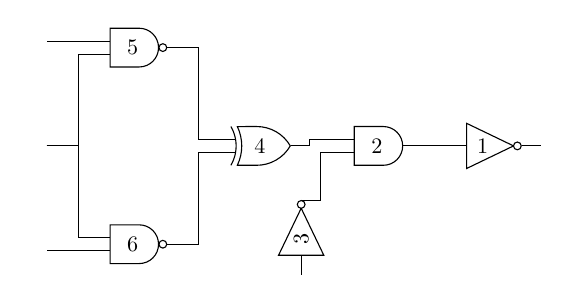
\begin{tikzpicture}[circuit logic US, scale=0.8]
    \node (i0) at (0,0) {}; 
    \node (i1) [below = of i0]{};
    \node (i2) [below = of i1]{};
    \node [nand gate, right=of i0] (n1) {5};
    \node [xor gate, right=3cm of i1] (x1) {4};
    \node [nand gate, right=of i2] (n2) {6};
    \node [and gate, right=of x1] (a1) {2};
    \node [not gate, right=of a1] (in1) {1};
    \node [not gate, rotate=90, below left=of a1] (in2) {3};

    %\draw (i0.east) -- ++(right:3mm) |- (n1.input 1);
    \draw (n1.input 1) -- ++(left:10mm);
    \draw (i1.east) -- ++(right:5mm) |- (n1.input 2);
    \draw (i1.east) -- ++(right:5mm) |- (n2.input 1);
    %\draw (i2.east) -- ++(right:3mm) |- (n2.input 2);
    \draw (n2.input 2) -- ++(left:10mm);

    \draw (n1.output) -- ++(right:5mm) |- (x1.input 1);
    \draw (n2.output) -- ++(right:5mm) |- (x1.input 2);
    \draw (x1.output) -- ++(right:3mm) |- (a1.input 1);
    \draw (in2.output) -- ++(right:3mm) |- (a1.input 2);

    \draw (a1.output) -- ++(right:3mm) |- (in1.input);
    \draw (in1.output) -- ++(right:3mm);
    \draw (in2.input) -- ++(down:3mm);
  \end{tikzpicture}
 }
 \subfloat[Modeled as graph] {
  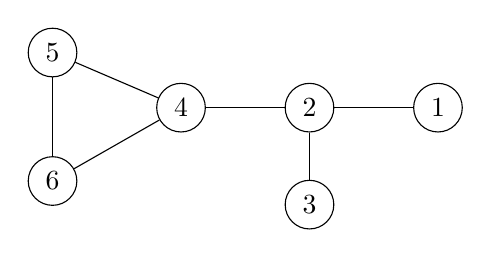
\begin{tikzpicture}
    [every node/.style={draw, circle}]
    \node (n5) {5};
    \node (n6) [below =of n5] {6};
    \node (n4) [right =of n5, yshift=-7mm] {4};
    \node (n2) [right =of n4] {2};
    \node (n3) [below =of n2, yshift=4mm] {3};
    \node (n1) [right =of n2] {1};

    \draw[-] (n5) -- (n6);
    \draw (n5) -- (n4);
    \draw (n4) -- (n6);
    \draw (n4) -- (n2);
    \draw (n2) -- (n3);
    \draw (n2) -- (n1);

  \end{tikzpicture}
  }
\end{figure}

  Now one can state a generic partitioning problem.

  \begin{problem}[40]

    Given a graph $G(V,E)$ where each vertex $v \in V$ has a size $s(v)$, and
    each edge $e \in E$ has a weight $w(e)$, the problem is to divide the set
    $V$ into $k$ subsets $V_1,\ldots,V_k$ such that an objective function is
    optimized, subject to certain constraints.

  \end{problem}

  One can formulate various constraints. Better known among them the listed
  below.

  \begin{description}
  \item [Bounded size] Assume that a single chip does not allow more than 6
  gates on average and your design has 100 of gates. Thus, you need to partition
  your circuit into at least 17 subsets, each of them is not having more than 6
  gates. Wouldn't be great if each partition have equal number of gates?

  \item[Minimize external wiring] Another situation is that we have many
  packages but there is a need to connect these packages through external wires.
  It is hightly desirable to minimize the lenght of external wiring (why?). 

  \end{description}

  One of the most popular algorithm to partitioning problem is due to
  \textbf{Keninghan and Lin} which finds a partition and improves it further.
  A heuristic is due known as \textbf{Fiduccia Mattheyses}. Some of the most
  powerful algorithm are based on a technique known as \textbf{simulated
  annealing}.
  
\subsection{Placement and routing problem}

  TODO : Give a small description and points to well known algorithms.

  \begin{description}
  \item [Grid routing]
  \item [Channel routing]
  \item [Layout generation]
  \item [Floorplanning]
  \end{description}

\subsection{Verification, validation and testing}

Following is from course notes provided by Prof. Madhav P. Desai, Verification
of VLSI circuits, 2010.

\begin{quotation}
"
Testing, verification and validation are critical processes in ensuring that the
circuit that is being manufactured meets the requirements that motivated its
design.

\begin{itemize}

\item By \textbf{testing}, we normally refer to the process used to determine
that the manufactured circuit is functional. Every manufactured circuit needs to
be tested, and the result of the test should, with a high degree of confidence,
determine that the circuit is functional.

\item By \textbf{verification}, we normally refer to the process used to confirm
that refinements in the design process are consistent with the circuit
specifica- tion. For example, when a logic circuit is implemented using
transistors, we need to verify that the transistor network is equivalent to the
logic circuit which it is supposed to implement. This is done at each refinement
step in the design process.

\item By \textbf{validation}, we normally refer to the process used to confirm
that a functional manufactured circuit will fulfill the requirements to which it
was designed. This usually involves the construction of a prototype and a test
setup which mimics reality to the maximum extent possible.  

\end{itemize}

Typically, the effort needed to implement these processes in the design of
complex circuits is substantial; a major fraction of the total product
development effort is contributed by the test, verification and validation
processes.  
"
\end{quotation}

Following are the major problems in testing.

\begin{itemize}

\item Manufacturing defects and fault models.  
\item The formulation of the test problem.  
\item The use of fault simulation in identifying fault coverage.  
\item Test pattern generation for combinational gate-level circuits using the
stuck-at fault model.  
\item Testing of sequential circuits.  
\item The use of scan techniques to test sequential circuits.  
\item Built-in self-test (BIST).  
\item Error correction and schemes for constructing fault-tolerant circuits. 
\end{itemize}

Verification is often done using simulation but this is not enough these days.
Use of formal verification is rising.
\begin{description}

\item[Formal Verification of combinational circuits] Given
a circtuit, prove some properties holds on it. To do it, we may use Binary decision diagrams
or Satisfiability solvers. 

\item [Formal verification of sequential circuits]  Given a state machine, prove
that some properties holds at a given time. Prove that given two designs or two
state machines are equivalent. State exploration techniques, model
checking techniques

\end{description}

\paragraph{Fault diagnosis}

  Refer to lecture notes. To be updated.


\section{Automata}

  


\end{document}          
